\documentclass[]{article}

\usepackage[a4paper]{geometry}
\usepackage{cite}
\usepackage{caption}
\usepackage{graphicx}
\usepackage{epstopdf}
\usepackage{booktabs}
\usepackage{amsmath}
\usepackage{subcaption}
\usepackage[section]{placeins}
\usepackage{changepage}
\usepackage{nicefrac}
\usepackage{pdfcomment}
\usepackage{comment}
\usepackage{hyperref}
\usepackage{array}

\begin{document}
	
\title{Derivation of the Finite Difference Frequency Domain (FDFD) Eigenequations}
\author{Ralf Mouthaan}
\date{October 2021}
\maketitle

\section{Introduction}

Following Yu \& Chang \cite{Yu2004}, we obtain two matrix equations.

\begin{equation}
-i \omega \mu_0
\begin{pmatrix}
\mathbf{H_x} \\
\mathbf{H_y} \\
\mathbf{H_z}
\end{pmatrix}
=
\begin{pmatrix}
\mathbf{0} & i \beta \mathbf{I} & \mathbf{A_y} \\
-i \beta \mathbf{I} & \mathbf{0} & -\mathbf{A_x} \\
-\mathbf{B_y} & \mathbf{B_x} & \mathbf{0}
\end{pmatrix}
\begin{pmatrix}
\mathbf{E_x} \\
\mathbf{E_y} \\
\mathbf{E_z}
\end{pmatrix}
\label{eq:FiniteDiffMatrixa}
\end{equation}

\begin{equation}
i \omega \epsilon_0
\begin{pmatrix}
\mathbf{\epsilon_{rx}} & \mathbf{0} & \mathbf{0} \\
\mathbf{0} & \mathbf{\epsilon_{ry}} & \mathbf{0} \\
\mathbf{0} & \mathbf{0} & \mathbf{\epsilon_{rz}}
\end{pmatrix}
\begin{pmatrix}
\mathbf{E_x} \\
\mathbf{E_y} \\
\mathbf{E_z}
\end{pmatrix}
=
\begin{pmatrix}
\mathbf{0} & i \beta \mathbf{I} & \mathbf{C_y} \\
-i \beta \mathbf{I} & \mathbf{0} & -\mathbf{C_x} \\
-\mathbf{D_y} & \mathbf{D_x} & \mathbf{0} 
\end{pmatrix}
\begin{pmatrix}
\mathbf{H_x} \\
\mathbf{H_y} \\
\mathbf{H_z}
\end{pmatrix}
\label{eq:FiniteDiffMatrixb}
\end{equation}

These are used to derive the following eigenequation.

\begin{equation}
\begin{pmatrix}
\mathbf{Q_{xx}} & \mathbf{Q_{xy}} \\
\mathbf{Q_{yx}} & \mathbf{Q_{yy}}
\end{pmatrix}
\begin{pmatrix}
\mathbf{H_x} \\
\mathbf{H_y}
\end{pmatrix}
=
\beta^2
\begin{pmatrix}
\mathbf{H_x} \\
\mathbf{H_y}
\end{pmatrix}
\label{eq:YuChangEigenEquation}
\end{equation}

where 

\begin{align*}
\mathbf{Q_{xx}} &= -k_0^{-2} \mathbf{A_x} \mathbf{D_y} \mathbf{C_x} \mathbf{\epsilon_{rz}}^{-1} \mathbf{B_y} + (\mathbf{\epsilon_{ry}} + k_0^{-2} \mathbf{A_x} \mathbf{D_x}) (k_0^2 \mathbf{I} + \mathbf{C_y} \mathbf{\epsilon_{rz}}^{-1} \mathbf{B_y}) \\
\mathbf{Q_{xy}} &= -(\mathbf{\epsilon_{ry}} + k_0^{-2} \mathbf{A_x}\mathbf{D_x}) \mathbf{C_y} \mathbf{\epsilon_{rz}}^{-1} \mathbf{B_x} + k_0^{-2} \mathbf{A_x} \mathbf{D_y} (k_0^2 \mathbf{I} + \mathbf{C_x} \mathbf{\epsilon_{rz}}^{-1} \mathbf{B_x}) \\
\mathbf{Q_{yy}} &= -k_0^{-2} \mathbf{A_y} \mathbf{D_x} \mathbf{C_y} \mathbf{\epsilon_{rz}}^{-1} \mathbf{B_x} + (\mathbf{\epsilon_{rx}} + k_0^{-2} \mathbf{A_y} \mathbf{D_y}) (k_0^2 \mathbf{I} + \mathbf{C_x} \mathbf{\epsilon_{rz}}^{-1} \mathbf{B_x}) \\
\mathbf{Q_{yx}} &= -(\mathbf{\epsilon_{rx}} + k_0^{-2} \mathbf{A_y}\mathbf{D_y}) \mathbf{C_x} \mathbf{\epsilon_{rz}}^{-1} \mathbf{B_y} + k_0^{-2} \mathbf{A_y} \mathbf{D_x} (k_0^2 \mathbf{I} + \mathbf{C_y} \mathbf{\epsilon_{rz}}^{-1} \mathbf{B_y})
\end{align*}

It is unclear how this eigenequation is derived. Yu \& Chang state ``After some mathematical work, an eigenvalue matrix equation in terms of the transverse magnetic fields can be obtained''. A similar expression is just given by Zhu \& Brown \cite{Zhu2002}, who state ``after some algebra, we obtain an eigenvalue equation in terms of transverse electric fields'' and also fail to give a derivation. Zhu \& Brown also given an eigenequation in terms of $\mathbf{E}$, but this cannot with perfectly matched layer absorbing boundary conditions. I want to investigate three things:

\begin{itemize}
	\item How Eq. \ref{eq:YuChangEigenEquation} is derived from Eqs. \ref{eq:FiniteDiffMatrixa} and \ref{eq:FiniteDiffMatrixb}
	\item How to derive a similar eigenequation in terms of $\mathbf{E}$
	\item Whether I can then set $\mathbf{E_x} = 0$ to obtain only linearly polarised modes.
\end{itemize}

\newpage

\section{Derivation of Eigenequation in terms of $\mathbf{H}$}


Taking Eq. \ref{eq:FiniteDiffMatrixb}, inverting the permittivities matrix and moving it to the other side gives us an expression for $\mathbf{E}$.

\begin{equation*}
\begin{pmatrix}
\mathbf{E_x} \\
\mathbf{E_y} \\
\mathbf{E_z}
\end{pmatrix}
=
-\frac{1}{i \omega \mu_0}
\begin{pmatrix}
\mathbf{0} & i \beta \mathbf{\epsilon_{rx}}^{-1} & \mathbf{\epsilon_{rx}}^{-1} \mathbf{C_y} \\
-i \beta \mathbf{\epsilon_{ry}}^{-1} & \mathbf{0} & - \mathbf{\epsilon_{ry}}^{-1} \mathbf{C_x} \\
-\mathbf{\epsilon_{rz}}^{-1} \mathbf{D_y} & \mathbf{\epsilon_{rz}}^{-1} \mathbf{D_x} & \mathbf{0} 
\end{pmatrix}
\begin{pmatrix}
\mathbf{H_x} \\
\mathbf{H_y} \\
\mathbf{H_z}
\end{pmatrix}
\end{equation*}

Inserting this into Eq. \ref{eq:FiniteDiffMatrixa}

\begin{equation*}
\omega^2 \epsilon_0 \mu_0
\begin{pmatrix}
\mathbf{H_x} \\
\mathbf{H_y} \\
\mathbf{H_z}
\end{pmatrix}
=
\begin{pmatrix}
\mathbf{0} & i \beta \mathbf{I} & \mathbf{A_y} \\
-i \beta \mathbf{I} & \mathbf{0} & -\mathbf{A_x} \\
-\mathbf{B_y} & \mathbf{B_x} & \mathbf{0}
\end{pmatrix}
\begin{pmatrix}
\mathbf{0} & i \beta \mathbf{\epsilon_{rx}}^{-1} & \mathbf{\epsilon_{rx}}^{-1} \mathbf{C_y} \\
-i \beta \mathbf{\epsilon_{ry}}^{-1} & \mathbf{0} & - \mathbf{\epsilon_{ry}}^{-1} \mathbf{C_x} \\
-\mathbf{\epsilon_{rz}}^{-1} \mathbf{D_y} & \mathbf{\epsilon_{rz}}^{-1} \mathbf{D_x} & \mathbf{0} 
\end{pmatrix}
\begin{pmatrix}
\mathbf{H_x} \\
\mathbf{H_y} \\
\mathbf{H_z}
\end{pmatrix}
\end{equation*}

Multiplying out the matrices, noting that $k_0^2 = \omega^2 \epsilon_0 \mu_0$

\begin{equation*}
k_0^2
\begin{pmatrix}
\mathbf{H_x} \\
\mathbf{H_y} \\
\mathbf{H_z}
\end{pmatrix}
=
\begin{pmatrix}
\beta^2 \mathbf{\epsilon_{ry}}^{-1} - \mathbf{A_y} \mathbf{\epsilon_{rz}}^{-1} \mathbf{D_y} 
&
\mathbf{A_y} \mathbf{\epsilon_{rz}}^{-1} \mathbf{D_x}
&
-i \beta \mathbf{\epsilon_{ry}}^{-1} \mathbf{C_x}
\\
\mathbf{A_x} \mathbf{\epsilon_{rz}}^{-1} \mathbf{D_y} 
& 
\beta^2 \mathbf{\epsilon_{rx}}^{-1} - \mathbf{A_x} \mathbf{\epsilon_{rz}}^{-1} \mathbf{D_x}
&
-i \beta \mathbf{\epsilon_{rx}}^{-1} \mathbf{C_y}
\\
-i \beta \mathbf{B_x} \mathbf{\epsilon_{ry}}^{-1}
& 
-i \beta \mathbf{B_y} \mathbf{\epsilon_{rx}}^{-1}
&
-\mathbf{B_y} \mathbf{\epsilon_{rx}}^{-1} \mathbf{C_y} - \mathbf{B_x} \mathbf{\epsilon_{ry}}^{-1} \mathbf{C_x}
\end{pmatrix}
\begin{pmatrix}
\mathbf{H_x} \\
\mathbf{H_y} \\
\mathbf{H_z}
\end{pmatrix}
\end{equation*}

Moving the LHS to the right such that we get an expression = 0, left-multiplying the top row by $\mathbf{B_x}$, left-multiplying the middle row by $\mathbf{B_y}$, and multiplying the bottom row by $-i \beta$

\begin{multline*}
\left(
\begin{matrix}
\beta^2 \mathbf{B_x} \mathbf{\epsilon_{ry}}^{-1} - \mathbf{B_x} \mathbf{A_y} \mathbf{\epsilon_{rz}}^{-1} \mathbf{D_y} - k_0^2 \mathbf{B_x} 
&
\mathbf{B_x} \mathbf{A_y} \mathbf{\epsilon_{rz}}^{-1} \mathbf{D_x}
\\
\mathbf{B_y} \mathbf{A_x} \mathbf{\epsilon_{rz}}^{-1} \mathbf{D_y} 
& 
\beta^2 \mathbf{B_y} \mathbf{\epsilon_{rx}}^{-1} - \mathbf{B_y} \mathbf{A_x} \mathbf{\epsilon_{rz}}^{-1} \mathbf{D_x} - k_0^2 \mathbf{B_y}
\\
-\beta^2 \mathbf{B_x} \mathbf{\epsilon_{ry}}^{-1}
& 
-\beta^2 \mathbf{B_y} \mathbf{\epsilon_{rx}}^{-1}
\end{matrix}
\right.
\\
\left.
\begin{matrix}
-i \beta \mathbf{B_x} \mathbf{\epsilon_{ry}}^{-1} \mathbf{C_x}
\\
-i \beta \mathbf{B_y} \mathbf{\epsilon_{rx}}^{-1} \mathbf{C_y}
\\
i \beta \mathbf{B_y} \mathbf{\epsilon_{rx}}^{-1} \mathbf{C_y} + i \beta \mathbf{B_x} \mathbf{\epsilon_{ry}}^{-1} \mathbf{C_x} + i \beta k_0^2 \mathbf{I}
\end{matrix}
\right)
\begin{pmatrix}
\mathbf{H_x} \\
\mathbf{H_y} \\
\mathbf{H_z}
\end{pmatrix}
=0
\end{multline*}

Add top and middle row to bottom row. Divide bottom row by $k_0^2$.

\begin{equation*}
\begin{pmatrix}
\beta^2 \mathbf{B_x} \mathbf{\epsilon_{ry}}^{-1} - \mathbf{B_x} \mathbf{A_y} \mathbf{\epsilon_{rz}}^{-1} \mathbf{D_y} - k_0^2 \mathbf{B_x} 
&
\mathbf{B_x} \mathbf{A_y} \mathbf{\epsilon_{rz}}^{-1} \mathbf{D_x}
&
-i \beta \mathbf{B_x} \mathbf{\epsilon_{ry}}^{-1} \mathbf{C_x}
\\
\mathbf{B_y} \mathbf{A_x} \mathbf{\epsilon_{rz}}^{-1} \mathbf{D_y} 
& 
\beta^2 \mathbf{B_y} \mathbf{\epsilon_{rx}}^{-1} - \mathbf{B_y} \mathbf{A_x} \mathbf{\epsilon_{rz}}^{-1} \mathbf{D_x} - k_0^2 \mathbf{B_y}
&
-i \beta \mathbf{B_y} \mathbf{\epsilon_{rx}}^{-1} \mathbf{C_y}
\\
k_0^{-2} (\mathbf{B_y} \mathbf{A_x} - \mathbf{B_x} \mathbf{A_y}) \mathbf{\epsilon_{rz}}^{-1} \mathbf{D_y} - \mathbf{B_x}
&
k_0^{-2} (\mathbf{B_x} \mathbf{A_y} - \mathbf{B_y} \mathbf{A_x}) \mathbf{\epsilon_{rz}}^{-1} \mathbf{D_x} - \mathbf{B_y}
&
i \beta \mathbf{I}
\end{pmatrix}
\begin{pmatrix}
\mathbf{H_x} \\
\mathbf{H_y} \\
\mathbf{H_z}
\end{pmatrix}
=0
\end{equation*}

Can now left-multiply top row by $\mathbf{\epsilon_{ry}} \mathbf{B_x}^{-1}$ and middle row by $\mathbf{\epsilon_{rx}} \mathbf{B_y}^{-1}$

\begin{equation*}
\begin{pmatrix}
\beta^2 - \mathbf{\epsilon_{ry}} \mathbf{A_y} \mathbf{\epsilon_{rz}}^{-1} \mathbf{D_y} - k_0^2 \mathbf{\epsilon_{ry}}
&
\mathbf{\epsilon_{ry}} \mathbf{A_y} \mathbf{\epsilon_{rz}}^{-1} \mathbf{D_x}
&
-i \beta \mathbf{C_x}
\\
\mathbf{\epsilon_{rx}}  \mathbf{A_x} \mathbf{\epsilon_{rz}}^{-1} \mathbf{D_y} 
& 
\beta^2 - \mathbf{\epsilon_{rx}} \mathbf{A_x} \mathbf{\epsilon_{rz}}^{-1} \mathbf{D_x} - k_0^2 \mathbf{\epsilon_{rx}}
&
-i \beta \mathbf{C_y}
\\
k_0^{-2} (\mathbf{B_y} \mathbf{A_x} - \mathbf{B_x} \mathbf{A_y}) \mathbf{\epsilon_{rz}}^{-1} \mathbf{D_y} - \mathbf{B_x}
&
k_0^{-2} (\mathbf{B_x} \mathbf{A_y} - \mathbf{B_y} \mathbf{A_x}) \mathbf{\epsilon_{rz}}^{-1} \mathbf{D_x} - \mathbf{B_y}
&
i \beta \mathbf{I}
\end{pmatrix}
\begin{pmatrix}
\mathbf{H_x} \\
\mathbf{H_y} \\
\mathbf{H_z}
\end{pmatrix}
=0
\end{equation*}

Taking the bottom row, right-multiplying by $\mathbf{C_x}$ and adding this to the top row. Taking the bottom row, right-multiplying by $\mathbf{C_y}$ and adding this to the second row. The $\mathbf{H_z}$ terms for the first two equations are now zero and can be dropped.

\begin{multline*}
\left(
\begin{matrix}
\beta^2 - \mathbf{\epsilon_{ry}} \mathbf{A_y} \mathbf{\epsilon_{rz}}^{-1} \mathbf{D_y} - k_0^2 \mathbf{\epsilon_{ry}} + k_0^{-2} (\mathbf{B_y} \mathbf{A_x} - \mathbf{B_x} \mathbf{A_y}) \mathbf{\epsilon_{rz}}^{-1} \mathbf{D_y} \mathbf{C_x} - \mathbf{B_x} \mathbf{C_x}
\\
\mathbf{\epsilon_{rx}}  \mathbf{A_x} \mathbf{\epsilon_{rz}}^{-1} \mathbf{D_y}  + k_0^{-2} (\mathbf{B_y} \mathbf{A_x} - \mathbf{B_x} \mathbf{A_y}) \mathbf{\epsilon_{rz}}^{-1} \mathbf{D_y} \mathbf{C_y} - \mathbf{B_x} \mathbf{C_y}
\end{matrix}
\right.
\\
\left.
\begin{matrix}
\mathbf{\epsilon_{ry}} \mathbf{A_y} \mathbf{\epsilon_{rz}}^{-1} \mathbf{D_x} + k_0^{-2} (\mathbf{B_x} \mathbf{A_y} - \mathbf{B_y} \mathbf{A_x}) \mathbf{\epsilon_{rz}}^{-1} \mathbf{D_x} \mathbf{C_x} - \mathbf{B_y} \mathbf{C_x}
\\
\beta^2 - \mathbf{\epsilon_{rx}} \mathbf{A_x} \mathbf{\epsilon_{rz}}^{-1} \mathbf{D_x} - k_0^2 \mathbf{\epsilon_{rx}}  + k_0^{-2} (\mathbf{B_x} \mathbf{A_y} - \mathbf{B_y} \mathbf{A_x}) \mathbf{\epsilon_{rz}}^{-1} \mathbf{D_x} \mathbf{C_y} - \mathbf{B_y} \mathbf{C_y}
\end{matrix}
\right)
\begin{pmatrix}
\mathbf{H_x} \\
\mathbf{H_y} \\
\end{pmatrix}
=0
\end{multline*}

Which gives the following eigenequation, where brackets have been expanded out and everything has been multiplied by -1 to make sure $\beta$ is positive.

\begin{multline}
\left(
\begin{matrix}
\mathbf{\epsilon_{ry}} \mathbf{A_y} \mathbf{\epsilon_{rz}}^{-1} \mathbf{D_y} + k_0^2 \mathbf{\epsilon_{ry}} - k_0^{-2} \mathbf{B_y} \mathbf{A_x} \mathbf{\epsilon_{rz}}^{-1} \mathbf{D_y} \mathbf{C_x} + k_0^{-2} \mathbf{B_x} \mathbf{A_y} \mathbf{\epsilon_{rz}}^{-1} \mathbf{D_y} \mathbf{C_x} + \mathbf{B_x} \mathbf{C_x}
\\
-\mathbf{\epsilon_{rx}}  \mathbf{A_x} \mathbf{\epsilon_{rz}}^{-1} \mathbf{D_y}  - k_0^{-2} \mathbf{B_y} \mathbf{A_x} \mathbf{\epsilon_{rz}}^{-1} \mathbf{D_y} \mathbf{C_y} + k_0^{-2} \mathbf{B_x} \mathbf{A_y} \mathbf{\epsilon_{rz}}^{-1} \mathbf{D_y} \mathbf{C_y} + \mathbf{B_x} \mathbf{C_y}
\end{matrix}
\right.
\\
\left.
\begin{matrix}
-\mathbf{\epsilon_{ry}} \mathbf{A_y} \mathbf{\epsilon_{rz}}^{-1} \mathbf{D_x} - k_0^{-2} \mathbf{B_x} \mathbf{A_y} \mathbf{\epsilon_{rz}}^{-1} \mathbf{D_x} \mathbf{C_x} + k_0^{-2} \mathbf{B_y} \mathbf{A_x} \mathbf{\epsilon_{rz}}^{-1} \mathbf{D_x} \mathbf{C_x} + \mathbf{B_y} \mathbf{C_x}
\\
\mathbf{\epsilon_{rx}} \mathbf{A_x} \mathbf{\epsilon_{rz}}^{-1} \mathbf{D_x} + k_0^2 \mathbf{\epsilon_{rx}}  - k_0^{-2} \mathbf{B_x} \mathbf{A_y} \mathbf{\epsilon_{rz}}^{-1} \mathbf{D_x} \mathbf{C_y} + k_0^{-2} \mathbf{B_y} \mathbf{A_x} \mathbf{\epsilon_{rz}}^{-1} \mathbf{D_x} \mathbf{C_y} + \mathbf{B_y} \mathbf{C_y}
\end{matrix}
\right)
\begin{pmatrix}
\mathbf{H_x} \\
\mathbf{H_y} \\
\end{pmatrix}
=
\beta^2
\begin{pmatrix}
\mathbf{H_x} \\
\mathbf{H_y} \\
\end{pmatrix}
\label{eq:HFieldEigenEquation}
\end{multline}

This is quite different from what was found by Yu \& Chang. Solving for the Erlangen PCF geometry and comparing the real components of the propagation constants obtained using Yu \& Chang's eigenequation (Eq. \ref{eq:YuChangEigenEquation}) with the real components of the propagation constants obtained using the H-field eigenequation (Eq. \ref{eq:HFieldEigenEquation}), we find that these agree to within $10^{-6}$ for the guided modes. The results are in agreement, and the equations seem to be somehow equivalent. It would still be interesting to know where Yu \& Chang's equation came from.

\begin{figure}[htb]
	\centering
	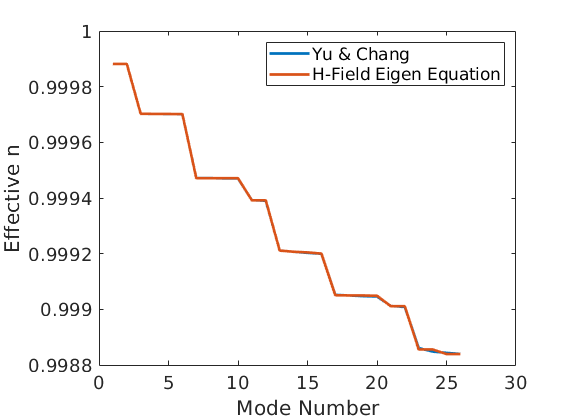
\includegraphics[width=0.6\textwidth]{Figures/YuChang_HFieldEigenEquation}
	\caption{Effective refractive index comparison between results obtained using Yu \& Chang's eigenequation (Eq. \ref{eq:YuChangEigenEquation}), and results obtained using the H-field eigenequation (Eq. \ref{eq:HFieldEigenEquation})}
\end{figure}

\newpage

\section{Derivation of the Eigenequation in terms of $\mathbf{E}$}

First, inserting the expression for $\mathbf{H}$ of Eq. \ref{eq:FiniteDiffMatrixa} into Eq. \ref{eq:FiniteDiffMatrixb}.

\begin{equation*}
k_0^2
\begin{pmatrix}
\mathbf{\epsilon_{rx}} & \mathbf{0} & \mathbf{0} \\
\mathbf{0} & \mathbf{\epsilon_{ry}} & \mathbf{0} \\
\mathbf{0} & \mathbf{0} & \mathbf{\epsilon_{rz}}
\end{pmatrix}
\begin{pmatrix}
\mathbf{E_x} \\
\mathbf{E_y} \\
\mathbf{E_z}
\end{pmatrix}
=
\begin{pmatrix}
\mathbf{0} & i \beta \mathbf{I} & \mathbf{C_y} \\
-i \beta \mathbf{I} & \mathbf{0} & -\mathbf{C_x} \\
-\mathbf{D_y} & \mathbf{D_x} & \mathbf{0} 
\end{pmatrix}
\begin{pmatrix}
\mathbf{0} & i \beta \mathbf{I} & \mathbf{A_y} \\
-i \beta \mathbf{I} & \mathbf{0} & -\mathbf{A_x} \\
-\mathbf{B_y} & \mathbf{B_x} & \mathbf{0}
\end{pmatrix}
\begin{pmatrix}
\mathbf{E_x} \\
\mathbf{E_y} \\
\mathbf{E_z}
\end{pmatrix}
\end{equation*}

Multiplying out the matrix on the right-hand side,

\begin{equation*}
k_0^2
\begin{pmatrix}
\mathbf{\epsilon_{rx}} & \mathbf{0} & \mathbf{0} \\
\mathbf{0} & \mathbf{\epsilon_{ry}} & \mathbf{0} \\
\mathbf{0} & \mathbf{0} & \mathbf{\epsilon_{rz}}
\end{pmatrix}
\begin{pmatrix}
\mathbf{E_x} \\
\mathbf{E_y} \\
\mathbf{E_z}
\end{pmatrix}
=
\begin{pmatrix}
\beta^2 \mathbf{I} - \mathbf{C_y}\mathbf{B_y}
&
\mathbf{C_y} \mathbf{B_x}
&
-i \beta \mathbf{A_x}
\\
\mathbf{C_x}\mathbf{B_y}
&
\beta^2 \mathbf{I} - \mathbf{C_x}\mathbf{B_x}
&
-i \beta \mathbf{A_y}
\\
-i \beta \mathbf{D_x}
&
-i \beta \mathbf{D_y}
&
-\mathbf{D_y} \mathbf{A_y} - \mathbf{D_x}\mathbf{A_x}
\end{pmatrix}
\begin{pmatrix}
\mathbf{E_x} \\
\mathbf{E_y} \\
\mathbf{E_z}
\end{pmatrix}
\end{equation*}

Left-multiply by the inverse permittivity matrix

\begin{equation*}
k_0^2
\begin{pmatrix}
\mathbf{E_x} \\
\mathbf{E_y} \\
\mathbf{E_z}
\end{pmatrix}
=
\begin{pmatrix}
\beta^2 \mathbf{\epsilon_{rx}}^{-1}- \mathbf{\epsilon_{rx}}^{-1} \mathbf{C_y}\mathbf{B_y}
&
\mathbf{\epsilon_{rx}}^{-1} \mathbf{C_y} \mathbf{B_x}
&
-i \beta \mathbf{\epsilon_{rx}}^{-1} \mathbf{A_x}
\\
\mathbf{\epsilon_{ry}}^{-1} \mathbf{C_x}\mathbf{B_y}
&
\beta^2 \mathbf{\epsilon_{ry}}^{-1} - \mathbf{\epsilon_{ry}}^{-1} \mathbf{C_x}\mathbf{B_x}
&
-i \beta \mathbf{\epsilon_{ry}}^{-1} \mathbf{A_y}
\\
-i \beta \mathbf{\epsilon_{rz}}^{-1} \mathbf{D_x}
&
-i \beta \mathbf{\epsilon_{rz}}^{-1} \mathbf{D_y}
&
-\mathbf{\epsilon_{rz}}^{-1} \mathbf{D_y} \mathbf{A_y} - \mathbf{\epsilon_{rz}}^{-1} \mathbf{D_x}\mathbf{A_x}
\end{pmatrix}
\begin{pmatrix}
\mathbf{E_x} \\
\mathbf{E_y} \\
\mathbf{E_z}
\end{pmatrix}
\end{equation*}

Move $k_0^2$ to the left to get a matrix equation = 0

\begin{equation*}
\begin{pmatrix}
\beta^2 \mathbf{\epsilon_{rx}}^{-1} - \mathbf{\epsilon_{rx}}^{-1} \mathbf{C_y}\mathbf{B_y} - k_0^2
&
\mathbf{\epsilon_{rx}}^{-1} \mathbf{C_y} \mathbf{B_x}
&
-i \beta \mathbf{\epsilon_{rx}}^{-1} \mathbf{A_x}
\\
\mathbf{\epsilon_{ry}}^{-1} \mathbf{C_x}\mathbf{B_y}
&
\beta^2 \mathbf{\epsilon_{ry}}^{-1} - \mathbf{\epsilon_{ry}}^{-1} \mathbf{C_x}\mathbf{B_x} - k_0^2
&
-i \beta \mathbf{\epsilon_{ry}}^{-1} \mathbf{A_y}
\\
-i \beta \mathbf{\epsilon_{rz}}^{-1} \mathbf{D_x}
&
-i \beta \mathbf{\epsilon_{rz}}^{-1} \mathbf{D_y}
&
-\mathbf{\epsilon_{rz}}^{-1} \mathbf{D_y} \mathbf{A_y} - \mathbf{\epsilon_{rz}}^{-1} \mathbf{D_x}\mathbf{A_x} - k_0^2
\end{pmatrix}
\begin{pmatrix}
\mathbf{E_x} \\
\mathbf{E_y} \\
\mathbf{E_z}
\end{pmatrix}
=0
\end{equation*}

Multiply top row by $\mathbf{D_x} \mathbf{\epsilon_{rx}}$; Multiply middle row by $\mathbf{D_y} \mathbf{\epsilon_{ry}}$;  Multiply bottom row by $-i \beta$

\begin{equation*}
\begin{pmatrix}
\beta^2 \mathbf{D_x} - \mathbf{D_x} \mathbf{C_y} \mathbf{B_y} - k_0^2 \mathbf{D_x} \mathbf{\epsilon_{rx}}
&
\mathbf{D_x} \mathbf{C_y} \mathbf{B_x}
&
-i \beta \mathbf{D_x} \mathbf{A_x}
\\
\mathbf{D_y} \mathbf{C_x} \mathbf{B_y}
&
\beta^2 \mathbf{D_y} - \mathbf{D_y} \mathbf{C_x}\mathbf{B_x} - k_0^2 \mathbf{D_y} \mathbf{\epsilon_{ry}} 
&
-i \beta \mathbf{D_y} \mathbf{A_y}
\\
-\beta^2 \mathbf{D_x}
&
-\beta^2 \mathbf{D_y}
&
i \beta \mathbf{D_y} \mathbf{A_y} + i \beta \mathbf{D_x}\mathbf{A_x} + i \beta k_0^2 \mathbf{\epsilon_{rz}}
\end{pmatrix}
\begin{pmatrix}
\mathbf{E_x} \\
\mathbf{E_y} \\
\mathbf{E_z}
\end{pmatrix}
=0
\end{equation*}

Add top and middle row to bottom row

\begin{equation*}
\begin{pmatrix}
\beta^2 \mathbf{D_x} - \mathbf{D_x} \mathbf{C_y} \mathbf{B_y} - k_0^2 \mathbf{D_x} \mathbf{\epsilon_{rx}}
&
\mathbf{D_x} \mathbf{C_y} \mathbf{B_x}
&
-i \beta \mathbf{D_x} \mathbf{A_x}
\\
\mathbf{D_y} \mathbf{C_x} \mathbf{B_y}
&
\beta^2 \mathbf{D_y} - \mathbf{D_y} \mathbf{C_x}\mathbf{B_x} - k_0^2 \mathbf{D_y} \mathbf{\epsilon_{ry}} 
&
-i \beta \mathbf{D_y} \mathbf{A_y}
\\
\mathbf{D_y} \mathbf{C_x} \mathbf{B_y} - \mathbf{D_x} \mathbf{C_y} \mathbf{B_y} - k_0^2 \mathbf{D_x} \mathbf{\epsilon_{rx}}
&
\mathbf{D_x} \mathbf{C_y} \mathbf{B_x} - \mathbf{D_y} \mathbf{C_x}\mathbf{B_x} - k_0^2 \mathbf{D_y} \mathbf{\epsilon_{ry}} 
&
i \beta k_0^2 \mathbf{\epsilon_{rz}}
\end{pmatrix}
\begin{pmatrix}
\mathbf{E_x} \\
\mathbf{E_y} \\
\mathbf{E_z}
\end{pmatrix}
=0
\end{equation*}

Left-multiply top row by $\mathbf{D_x}^{-1}$, left-multiply middle row by $\mathbf{D_y}^{-1}$, left multiply bottom row by $k_0^{-2} \mathbf{\epsilon_{rz}}^{-1}$

\begin{multline*}
\left(
\begin{matrix}
\beta^2 - \mathbf{C_y} \mathbf{B_y} - k_0^2 \mathbf{\epsilon_{rx}}
\\
\mathbf{C_x} \mathbf{B_y}
\\
k_0^{-2} \mathbf{\epsilon_{rz}}^{-1} \mathbf{D_y} \mathbf{C_x} \mathbf{B_y} - k_0^{-2} \mathbf{\epsilon_{rz}}^{-1} \mathbf{D_x} \mathbf{C_y} \mathbf{B_y} -  \mathbf{\epsilon_{rz}}^{-1} \mathbf{D_x} \mathbf{\epsilon_{rx}}
\end{matrix}
\right.
\\
\left.
\begin{matrix}
\mathbf{C_y} \mathbf{B_x}
&
-i \beta \mathbf{A_x}
\\
\beta^2 - \mathbf{C_x} \mathbf{B_x} - k_0^2  \mathbf{\epsilon_{ry}} 
&
-i \beta \mathbf{A_y}
\\
k_0^{-2} \mathbf{\epsilon_{rz}}^{-1} \mathbf{D_x} \mathbf{C_y} \mathbf{B_x} - k_0^{-2} \mathbf{\epsilon_{rz}}^{-1} \mathbf{D_y} \mathbf{C_x}\mathbf{B_x} - \mathbf{\epsilon_{rz}}^{-1} \mathbf{D_y} \mathbf{\epsilon_{ry}} 
&
i \beta \mathbf{I}
\end{matrix}
\right)
\begin{pmatrix}
\mathbf{E_x} \\
\mathbf{E_y} \\
\mathbf{E_z}
\end{pmatrix}
=0
\end{multline*}

Add $\mathbf{A_x}$ times bottom row to top row. Add $\mathbf{A_y}$ times bottom row to middle row. We can now consider only the $\mathbf{E_x}$ and $\mathbf{E_y}$ components.

\begin{multline*}
\left(
\begin{matrix}
\beta^2 - \mathbf{C_y} \mathbf{B_y} - k_0^2 \mathbf{\epsilon_{rx}} + k_0^{-2} \mathbf{A_x} \mathbf{\epsilon_{rz}}^{-1} \mathbf{D_y} \mathbf{C_x} \mathbf{B_y} - k_0^{-2} \mathbf{A_x} \mathbf{\epsilon_{rz}}^{-1} \mathbf{D_x} \mathbf{C_y} \mathbf{B_y} -  \mathbf{A_x} \mathbf{\epsilon_{rz}}^{-1} \mathbf{D_x} \mathbf{\epsilon_{rx}}
\\
\mathbf{C_x} \mathbf{B_y} + k_0^{-2} \mathbf{A_y} \mathbf{\epsilon_{rz}}^{-1} \mathbf{D_y} \mathbf{C_x} \mathbf{B_y} - k_0^{-2} \mathbf{A_y} \mathbf{\epsilon_{rz}}^{-1} \mathbf{D_x} \mathbf{C_y} \mathbf{B_y} -  \mathbf{A_y} \mathbf{\epsilon_{rz}}^{-1} \mathbf{D_x} \mathbf{\epsilon_{rx}}
\end{matrix}
\right.
\\
\left.
\begin{matrix}
\mathbf{C_y} \mathbf{B_x} + k_0^{-2} \mathbf{A_x} \mathbf{\epsilon_{rz}}^{-1} \mathbf{D_x} \mathbf{C_y} \mathbf{B_x} - k_0^{-2} \mathbf{A_x} \mathbf{\epsilon_{rz}}^{-1} \mathbf{D_y} \mathbf{C_x}\mathbf{B_x} - \mathbf{A_x} \mathbf{\epsilon_{rz}}^{-1} \mathbf{D_y} \mathbf{\epsilon_{ry}} 
\\
\beta^2 - \mathbf{C_x} \mathbf{B_x} - k_0^2  \mathbf{\epsilon_{ry}} + k_0^{-2} \mathbf{A_y} \mathbf{\epsilon_{rz}}^{-1} \mathbf{D_x} \mathbf{C_y} \mathbf{B_x} - k_0^{-2} \mathbf{A_y} \mathbf{\epsilon_{rz}}^{-1} \mathbf{D_y} \mathbf{C_x}\mathbf{B_x} - \mathbf{A_y} \mathbf{\epsilon_{rz}}^{-1} \mathbf{D_y} \mathbf{\epsilon_{ry}} 
\end{matrix}
\right)
\begin{pmatrix}
\mathbf{E_x} \\
\mathbf{E_y}
\end{pmatrix}
=0
\end{multline*}

Moving the $\beta^2$ turn to the other side and multiplying by -1 to give an eigenequation.

\begin{multline}
\left(
\begin{matrix}
\mathbf{C_y} \mathbf{B_y} + k_0^2 \mathbf{\epsilon_{rx}} - k_0^{-2} \mathbf{A_x} \mathbf{\epsilon_{rz}}^{-1} \mathbf{D_y} \mathbf{C_x} \mathbf{B_y} + k_0^{-2} \mathbf{A_x} \mathbf{\epsilon_{rz}}^{-1} \mathbf{D_x} \mathbf{C_y} \mathbf{B_y} +  \mathbf{A_x} \mathbf{\epsilon_{rz}}^{-1} \mathbf{D_x} \mathbf{\epsilon_{rx}}
\\
-\mathbf{C_x} \mathbf{B_y} - k_0^{-2} \mathbf{A_y} \mathbf{\epsilon_{rz}}^{-1} \mathbf{D_y} \mathbf{C_x} \mathbf{B_y} + k_0^{-2} \mathbf{A_y} \mathbf{\epsilon_{rz}}^{-1} \mathbf{D_x} \mathbf{C_y} \mathbf{B_y} +  \mathbf{A_y} \mathbf{\epsilon_{rz}}^{-1} \mathbf{D_x} \mathbf{\epsilon_{rx}}
\end{matrix}
\right.
\\
\left.
\begin{matrix}
-\mathbf{C_y} \mathbf{B_x} - k_0^{-2} \mathbf{A_x} \mathbf{\epsilon_{rz}}^{-1} \mathbf{D_x} \mathbf{C_y} \mathbf{B_x} + k_0^{-2} \mathbf{A_x} \mathbf{\epsilon_{rz}}^{-1} \mathbf{D_y} \mathbf{C_x}\mathbf{B_x} + \mathbf{A_x} \mathbf{\epsilon_{rz}}^{-1} \mathbf{D_y} \mathbf{\epsilon_{ry}} 
\\
\mathbf{C_x} \mathbf{B_x} + k_0^2  \mathbf{\epsilon_{ry}} - k_0^{-2} \mathbf{A_y} \mathbf{\epsilon_{rz}}^{-1} \mathbf{D_x} \mathbf{C_y} \mathbf{B_x} + k_0^{-2} \mathbf{A_y} \mathbf{\epsilon_{rz}}^{-1} \mathbf{D_y} \mathbf{C_x}\mathbf{B_x} + \mathbf{A_y} \mathbf{\epsilon_{rz}}^{-1} \mathbf{D_y} \mathbf{\epsilon_{ry}} 
\end{matrix}
\right)
\begin{pmatrix}
\mathbf{E_x} \\
\mathbf{E_y}
\end{pmatrix}
=\beta^2
\begin{pmatrix}
\mathbf{E_x} \\
\mathbf{E_y}
\end{pmatrix}
\label{eq:EFieldEigenEquation}
\end{multline}

Modelling the Erlangen PCF geometry using Yu \& Chang's eigenequation (Eq. \ref{eq:YuChangEigenEquation}) as well as the E-field eigenequation (Eq. \ref{eq:EFieldEigenEquation}) again gives good agreement.

\begin{figure}[htb]
	\centering
	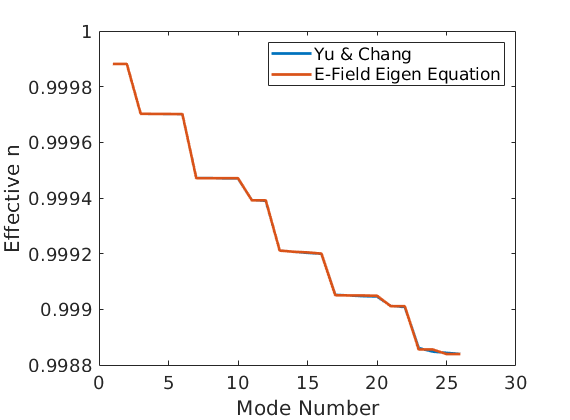
\includegraphics[width=0.6\textwidth]{Figures/YuChang_EFieldEigenEquation}
	\caption{Effective refractive index comparison between results obtained using Yu \& Chang's eigenequation (Eq. \ref{eq:YuChangEigenEquation}), and results obtained using the E-field eigenequation (Eq. \ref{eq:EFieldEigenEquation})}
\end{figure}

It is noted that $\mathbf{A_x}$, $\mathbf{A_y}$, $\mathbf{B_x}$, $\mathbf{B_y}$, $\mathbf{C_x}$, $\mathbf{C_y}$, $\mathbf{D_x}$ and $\mathbf{D_y}$ have strong similarities, and $\mathbf{\epsilon_{rx}}$, $\mathbf{\epsilon_{ry}}$, $\mathbf{\epsilon_{rz}}$ are identical for this geometry, and so it is still possible that the equation is not quite correct, but I am getting good results in this case.

\newpage

\section{Derivation of LP Eigenequation}

To solve for the linearly polarised mode where $\mathbf{E_x} = 0$ we only need to consider the bottom-right matrix element of the eigenequation in $\mathbf{E}$

\begin{equation}
\begin{pmatrix}
-\mathbf{C_x} \mathbf{B_x} + k_0^2  \mathbf{\epsilon_{ry}} - k_0^{-2} \mathbf{A_y} \mathbf{\epsilon_{rz}}^{-1} \mathbf{D_x} \mathbf{C_y} \mathbf{B_x} + k_0^{-2} \mathbf{A_y} \mathbf{\epsilon_{rz}}^{-1} \mathbf{D_y} \mathbf{C_x}\mathbf{B_x} + \mathbf{A_y} \mathbf{\epsilon_{rz}}^{-1} \mathbf{D_y} \mathbf{\epsilon_{ry}} 
\end{pmatrix}
\mathbf{E_y}
=\beta^2
\mathbf{E_y}
\label{eq:LPEigenEquation}
\end{equation}

Modelling the Erlangen PCF geometry using Yu \& Chang's eigenequation (Eq. \ref{eq:YuChangEigenEquation}) as well as the LP eigenequation (Eq. \ref{eq:EFieldEigenEquation}) again gives good agreement. Here, we have only considered every second mode given by Yu \& Chang's technique, so that polarisation degenerate modes are skipped.

\begin{figure}[htb]
	\centering
	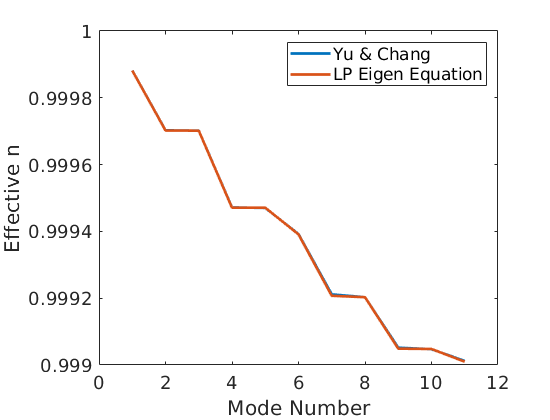
\includegraphics[width=0.6\textwidth]{Figures/YuChang_LPEigenEquation}
	\caption{Effective refractive index comparison between results obtained using Yu \& Chang's eigenequation (Eq. \ref{eq:YuChangEigenEquation}), and results obtained using the LP eigenequation (Eq. \ref{eq:LPEigenEquation})}
\end{figure}

Plotting out the modes obtained gives sensible results (Fig. \ref{fig:LPModePlots}). The solver also runs quicker, as might be expected. In this case, it takes 68s to solve for the LP modes, as opposed to 360s to solve for the vector modes.

\begin{figure}[htb]
	\centering
	\begin{subfigure}{0.3\textwidth}
		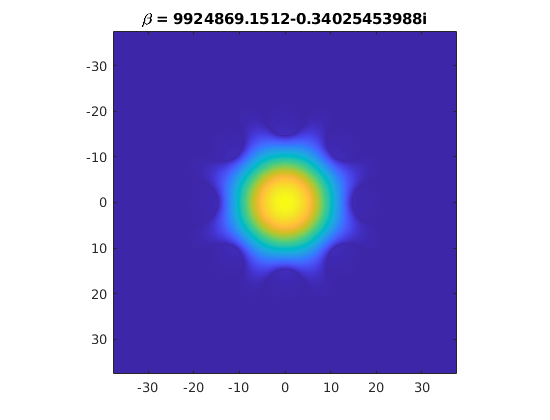
\includegraphics[width=\textwidth]{Figures/LP01}
	\end{subfigure}
	~
	\begin{subfigure}{0.3\textwidth}
		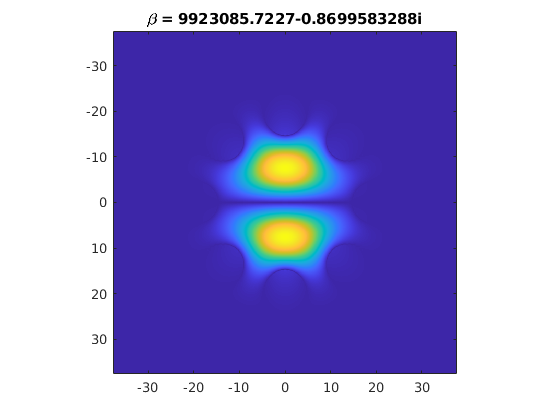
\includegraphics[width=\textwidth]{Figures/LP11a}
	\end{subfigure}
	~
	\begin{subfigure}{0.3\textwidth}
		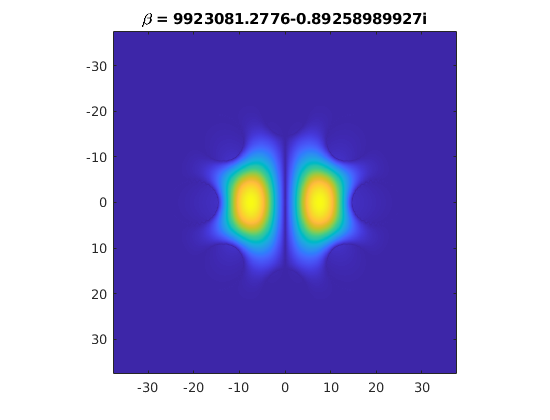
\includegraphics[width=\textwidth]{Figures/LP11b}
	\end{subfigure}
	\\
	\begin{subfigure}{0.3\textwidth}
		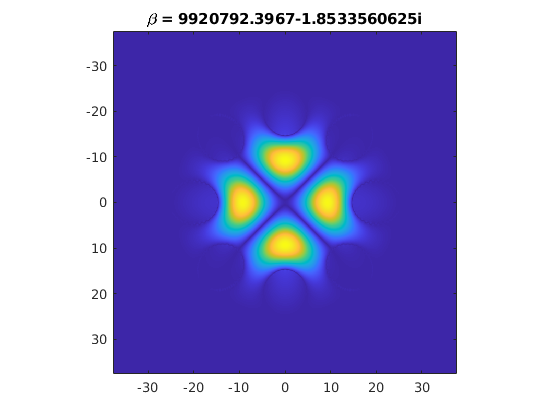
\includegraphics[width=\textwidth]{Figures/LP21a}
	\end{subfigure}
	~
	\begin{subfigure}{0.3\textwidth}
		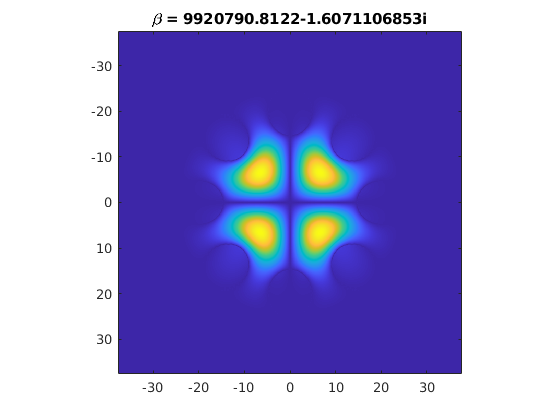
\includegraphics[width=\textwidth]{Figures/LP21b}
	\end{subfigure}
	~
	\begin{subfigure}{0.3\textwidth}
		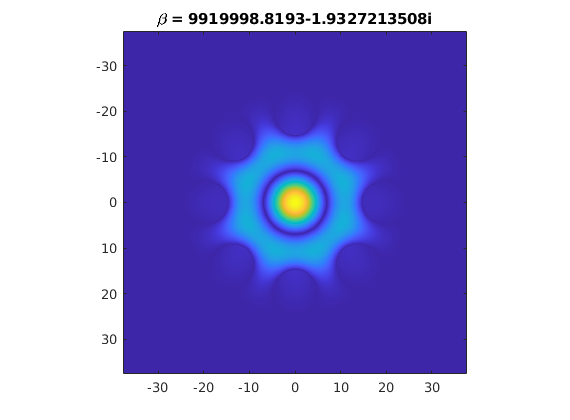
\includegraphics[width=\textwidth]{Figures/LP02}
	\end{subfigure}
	\\
	\begin{subfigure}{0.3\textwidth}
		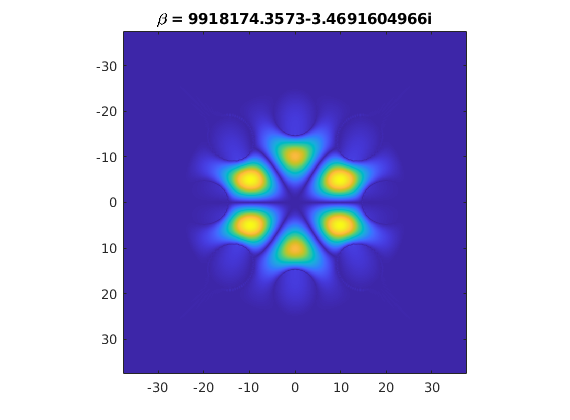
\includegraphics[width=\textwidth]{Figures/LP31a}
	\end{subfigure}
	~
	\begin{subfigure}{0.3\textwidth}
		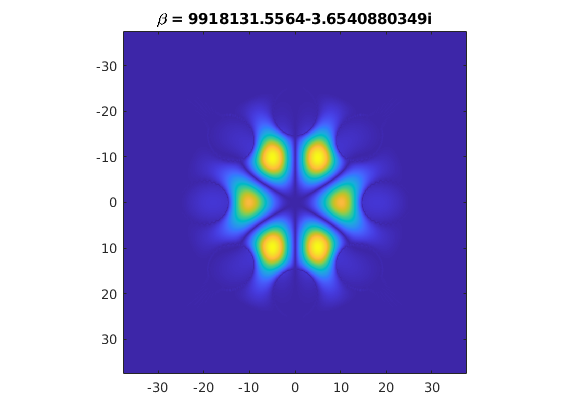
\includegraphics[width=\textwidth]{Figures/LP31b}
	\end{subfigure}
	~
	\begin{subfigure}{0.3\textwidth}
		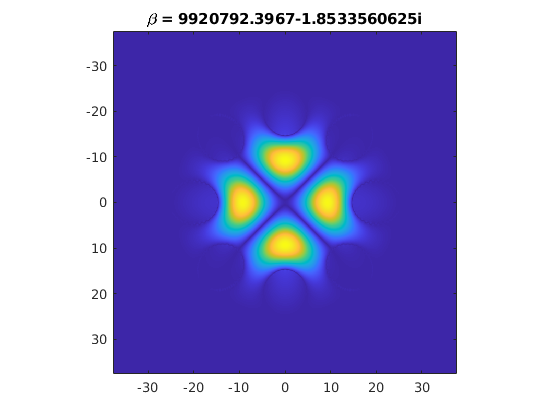
\includegraphics[width=\textwidth]{Figures/LP21a}
	\end{subfigure}
	\\
	\begin{subfigure}{0.3\textwidth}
		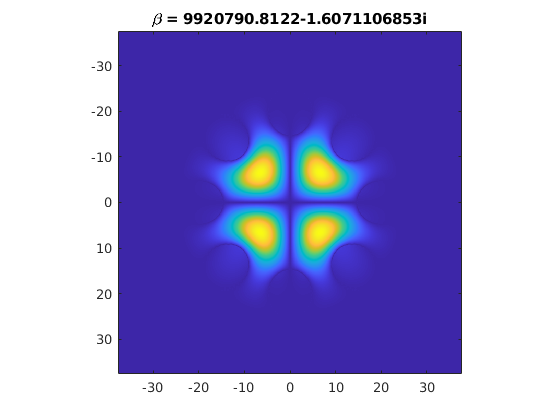
\includegraphics[width=\textwidth]{Figures/LP21b}
	\end{subfigure}
	~
	\begin{subfigure}{0.3\textwidth}
		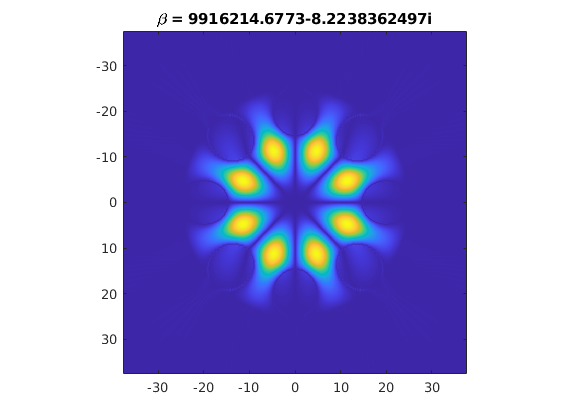
\includegraphics[width=\textwidth]{Figures/LP41}
	\end{subfigure}
	~
	\begin{subfigure}{0.3\textwidth}
		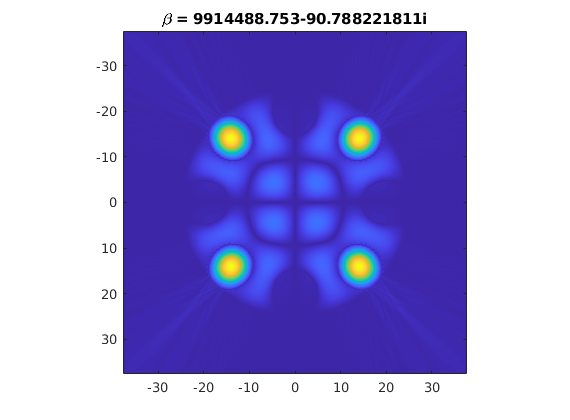
\includegraphics[width=\textwidth]{Figures/Non Guided}
	\end{subfigure}
\caption{LP modes obtained using Eq. \ref{eq:LPEigenEquation}}
\label{fig:LPModePlots}
\end{figure}

\begin{thebibliography}{9}
	\bibitem{Yu2004}
	Chin-Ping Yu and Hung-Chun Chang, "Yee-mesh-based finite difference eigenmode solver with PML absorbing boundary conditions for optical waveguides and photonic crystal fibers," Opt. Express 12, 6165-6177 (2004)
	
	\bibitem{Zhu2002}
	Zhaoming Zhu and Thomas G. Brown, "Full-vectorial finite-difference analysis of microstructured optical fibers," Opt. Express 10, 853-864 (2002)
\end{thebibliography}








	
\end{document}